\subsection{Geometry}
\subsubsection{Triangles}
Circumradius: $R=\dfrac{abc}{4A}$ , Inradius: $r=\dfrac{A}{s}$\\
Length of median (divides triangle into two equal-area triangles): $m_a=\tfrac{1}{2}\sqrt{2b^2+2c^2-a^2}$\\
Length of bisector (divides angles in two): $s_a=\sqrt{bc\left[1-\left(\dfrac{a}{b+c}\right)^2\right]}$\\
Law of tangents: $\dfrac{a+b}{a-b}=\dfrac{\tan\dfrac{\alpha+\beta}{2}}{\tan\dfrac{\alpha-\beta}{2}}$\\
\subsubsection{Quadrilaterals}
With side lengths $a,b,c,d$, diagonals $e, f$, diagonals angle $\theta$, area $A$ and
magic flux $F=b^2+d^2-a^2-c^2$:

\[ 4A = 2ef \cdot \sin\theta = F\tan\theta = \sqrt{4e^2f^2-F^2} \]

 For cyclic quadrilaterals the sum of opposite angles is $180^\circ$,
$ef = ac + bd$, and $A = \sqrt{(p-a)(p-b)(p-c)(p-d)}$.

\subsubsection{Spherical coordinates}
\centerline{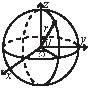
\includegraphics[width=25mm]{../code/sphericalCoordinates}}
\[\begin{array}{cc}
x = r\sin\theta\cos\phi & r = \sqrt{x^2+y^2+z^2}\\
y = r\sin\theta\sin\phi & \theta = \textrm{acos}(z/\sqrt{x^2+y^2+z^2})\\
z = r\cos\theta & \phi = \textrm{atan2}(y,x)
\end{array}\]

\subsection{Sums}
  1^2 + 2^2 + 3^2 + \dots + n^2 &= \frac{n(2n+1)(n+1)}{6} \\
  1^3 + 2^3 + 3^3 + \dots + n^3 &= \frac{n^2(n+1)^2}{4} \\
  1^4 + 2^4 + 3^4 + \dots + n^4 &= \frac{n(n+1)(2n+1)(3n^2 + 3n - 1)}{30} \\
  $\Scale[0.85]{ \sum\limits_{i=1}^{n} i^{m} = \frac{1}{m + 1}  \left[ (n + 1)^{m + 1} - 1 - \sum\limits_{i=1}^{n} \left((i+1)^{m+1} - i^{m+1} - (m + 1)i^{m}\right)\right]} $\\
  $\Scale[0.99]{\sum\limits_{i=1}^{n-1} i^{m} = \frac{1}{m + 1} \sum\limits_{k=0}^{m} { {m+1}\choose{k} } B_{k}n^{m + 1 - k}}$\\
  $\sum\limits_{k=0}^n kx^k = (x - (n+1)x^{n+1} + nx^{n+2})/(x-1)^2$


\subsection{Series}
$$e^x = 1+x+\frac{x^2}{2!}+\frac{x^3}{3!}+\dots,\,(-\infty<x<\infty)$$
$$\ln(1+x) = x-\frac{x^2}{2}+\frac{x^3}{3}-\frac{x^4}{4}+\dots,\,(-1<x\leq1)$$
$$\sqrt{1+x} = 1+\frac{x}{2}-\frac{x^2}{8}+\frac{2x^3}{32}-\frac{5x^4}{128}+\dots,\,(-1\leq x\leq1)$$
$$\sin x = x-\frac{x^3}{3!}+\frac{x^5}{5!}-\frac{x^7}{7!}+\dots,\,(-\infty<x<\infty)$$
$$\cos x = 1-\frac{x^2}{2!}+\frac{x^4}{4!}-\frac{x^6}{6!}+\dots,\,(-\infty<x<\infty)$$
$$(x + a)^{-n} = \sum\limits_{k=0}^{\infty} (-1)^{k} { {n + k - 1}\choose{k}} x^{k}a^{-n-k}$$

\subsection{Pythagorean Triples}
 The Pythagorean triples are uniquely generated by
 \[ a=k\cdot (m^{2}-n^{2}),\ \,b=k\cdot (2mn),\ \,c=k\cdot (m^{2}+n^{2}), \]
 with $m > n > 0$, $k > 0$, $m \bot n$, and either $m$ or $n$ even.


\subsection{Number Theory}
\subsubsection{Primes}
  $p=962592769$ is such that $2^{21} \mid p-1$, which may be useful. For hashing
  use 970592641 (31-bit number), 31443539979727 (45-bit), 3006703054056749
  (52-bit). There are 78498 primes less than 1\,000\,000.

  Primitive roots exist modulo any prime power $p^a$, except for $p = 2, a > 2$, and there are $\phi(\phi(p^a))$ many.
  For $p = 2, a > 2$, the group $\mathbb Z_{2^a}^\times$ is instead isomorphic to $\mathbb Z_2 \times \mathbb Z_{2^{a-2}}$.

\subsubsection{Estimates}
  $\sum_{d|n} d = O(n \log \log n)$.

  The number of divisors of $n$ is at most around 100 for $n < 5e4$, 500 for $n < 1e7$, 2000 for $n < 1e10$, 200\,000 for $n < 1e19$.

\subsubsection{Perfect numbers}  $n>1$ is called perfect if it equals
sum of its proper divisors and $1$.  Even $n$ is perfect iff $n = 2^{p-1} (2^p - 1)$
and $2^p - 1$ is prime (Mersenne's). No odd perfect numbers are yet found.

\subsubsection{Carmichael numbers}
A positive composite $n$ is a Carmichael number
($a^{n-1} \equiv 1 \pmod{n}$ for all $a$: $\gcd(a,n)=1$),
iff $n$ is square-free, and for all prime divisors $p$ of $n$, $p-1$ divides $n-1$.

\subsubsection{Mobius function}
$\mu(1) = 1$. $\mu(n) = 0$, if $n$ is not squarefree.
$\mu(n) = (-1)^s$, if $n$ is the product of $s$ distinct primes.
Let $f$, $F$ be functions on positive integers.
If for all $n \in N$, $F(n)=\sum_{d|n} f(d)$, then $f(n) = \sum_{d|n} \mu(d) F(\frac{n}{d})$,
and vice versa. \quad
$\phi(n) = \sum_{d|n} \mu(d) \frac{n}{d}$.
\quad $\sum_{d|n} \mu(d) = 1$. \\
If $f$ is multiplicative, then $\sum_{d|n} \mu(d) f(d) = \prod_{p|n}(1-f(p))$,
$\sum_{d|n} \mu(d)^2 f(d) = \prod_{p|n} (1+f(p))$.

\subsubsection{Legendre symbol} If $p$ is an odd prime, $a \in {\mathbb Z}$, then
$\left(\frac{a}{p}\right)$ equals $0$, if $p | a$; $1$ if $a$ is a quadratic
residue modulo $p$; and $-1$ otherwise.
Euler's criterion:
$\left(\frac{a}{p}\right)=a^{\left(\frac{p-1}{2}\right)} \pmod p$. \\
%$\left(\frac{a}{p}\right) \left(\frac{b}{p}\right) = \left(\frac{ab}{p}\right)$
%Law of Quadratic Reciprocity: for any distinct odd primes $p$ and $q$,
%$\left(\frac{p}{q}\right) \left(\frac{q}{p}\right) = (-1)^{\frac{p-1}{2} \cdot \frac{q-1}{2}}$
\subsubsection{Jacobi symbol}  %Generalization of Legendre's symbol to any odd modulus. \\
If $n=p_1^{a_1} \cdots p_k^{a_k}$ is odd, then
$\left(\frac{a}{n}\right) = \prod_{i=1}^k \left(\frac{a}{p_i}\right)^{k_i}$.

%\subsubsection{Kronecker symbol}
%Let $a$ be a positive integer, which is not a perfect square and
%$a \equiv 0$ or $1 {\pmod 4}$. \\
%$\left(\frac{a}{2}\right) = \{ 1$, if $a \equiv 1 {\pmod 8}$;
%$-1$, if $a \equiv 5 {\pmod 8} \}$. \\
%$\left(\frac{a}{n}\right) = \prod_{j=1}^k p_j^{k_j}$,
%if gcd$(a,n) \ne 1$ and $n=\prod p_i^{k_i}$.
%$\left(\frac{a}{n}\right)$ equals Jacobi symbol otherwise.

\subsubsection{Primitive roots}  If the order of $g$ modulo $m$ (min $n>0$:
$g^n \equiv 1 \pmod{m}$) is $\phi(m)$, then $g$ is called a primitive root.
If $Z_m$ has a primitive root, then it has $\phi(\phi(m))$ distinct primitive
roots. $Z_m$ has a primitive root iff $m$ is one of $2$, $4$,
$p^k$, $2p^k$, where $p$ is an odd prime.
If $Z_m$ has a primitive root $g$, then for all $a$ coprime to $m$,
there exists unique integer $i=\text{ind}_g(a)$ modulo $\phi(m)$,
such that $g^i \equiv a \pmod{m}$.
$\text{ind}_g(a)$ has logarithm-like properties:
$\text{ind}(1) = 0$, $\text{ind}(ab) = \text{ind}(a) + \text{ind}(b)$.

If $p$ is prime and $a$ is not divisible by $p$, then congruence
$x^n \equiv a \pmod{p}$ has $\gcd(n, p-1)$ solutions if
$a^{(p-1)/\gcd(n,p-1)} \equiv 1 \pmod{p}$, and no solutions otherwise.
(Proof sketch: let $g$ be a primitive root, and
$g^i \equiv a \pmod{p}$, $g^u \equiv x \pmod{p}$.
$x^n \equiv a \pmod{p}$ iff $g^{nu} \equiv g^i \pmod{p}$ iff $nu \equiv i \pmod{p}$.)

\subsubsection{Discrete logarithm problem}  Find $x$ from $a^x \equiv b \pmod{m}$.
Can be solved in $O(\sqrt{m})$ time and space with a meet-in-the-middle trick.
Let $n = \lceil \sqrt{m} \rceil$, and $x = ny - z$.
Equation becomes $a^{ny} \equiv b a^z \pmod{m}$.  Precompute all values that
the RHS can take for $z = 0, 1, \dots, n-1$, and brute force $y$ on the LHS,
each time checking whether there's a corresponding value for RHS.

\subsubsection{Pythagorean triples}  Integer solutions of $x^2 + y^2 = z^2$
All relatively prime triples are given by:
$x=2mn, y=m^2-n^2, z=m^2+n^2$ where $m>n, \gcd(m,n)=1$ and $m \not\equiv n \pmod{2}$.
All other triples are multiples of these.
Equation $x^2 + y^2 = 2z^2$ is equivalent to $(\frac{x+y}{2})^2 + (\frac{x-y}{2})^2 = z^2$.

\subsubsection{Postage stamps/McNuggets problem}  Let $a$, $b$ be relatively-prime integers.
There are exactly $\frac{1}{2}(a-1)(b-1)$ numbers \emph{not} of form $ax+by$ ($x,y \ge 0$),
and the largest is $(a-1)(b-1)-1 = ab - a - b$.

\subsubsection{Fermat's two-squares theorem}  Odd prime $p$ can be represented
as a sum of two squares iff $p \equiv 1 {\pmod 4}$.
A product of two sums of two squares is a sum of two squares.
Thus, $n$ is a sum of two squares iff every prime of
form $p=4k+3$ occurs an even number of times in $n$'s factorization.

% }}}

\subsection{Permutations}
  \subsubsection{Factorial}
    \begin{center}
\begin{tabular}{l}
\begin{tabular}{c|c@{\ }c@{\ }c@{\ }c@{\ }c@{\ }c@{\ }c@{\ }c@{\ }c@{\ }c}
$n$  & 1 & 2 & 3 & 4  & 5   & 6   & 7    & 8     & 9      & 10\\
\hline
$n!$ & 1 & 2 & 6 & 24 & 120 & 720 & 5040 & 40320 & 362880 & 3628800\\
\end{tabular}\\
\begin{tabular}{c|c@{\ }c@{\ }c@{\ }c@{\ }c@{\ }c@{\ }c@{\ }c@{\ }c@{\ }c}
$n$  & 11    & 12    & 13    & 14     & 15     & 16     & 17\\
\hline
$n!$ & 4.0e7 & 4.8e8 & 6.2e9 & 8.7e10 & 1.3e12 & 2.1e13 & 3.6e14\\
\end{tabular}\\
\begin{tabular}{c|c@{\ }c@{\ }c@{\ }c@{\ }c@{\ }c@{\ }c@{\ }c@{\ }c@{\ }c}
$n$  & 20   & 25   & 30   & 40   & 50   & 100   & 150   & 171\\
\hline
$n!$ & 2e18 & 2e25 & 3e32 & 8e47 & 3e64 & 9e157 & 6e262 & \scriptsize{$>$DBL\_MAX}\\
\end{tabular}
\end{tabular}
\end{center}


  \subsubsection{Cycles}
    Let $g_S(n)$ be the number of $n$-permutations whose cycle lengths all belong to the set $S$. Then
    $$\sum_{n=0} ^\infty g_S(n) \frac{x^n}{n!} = \exp\left(\sum_{n\in S} \frac{x^n} {n} \right)$$

  \subsubsection{Derangements}
    Permutations of a set such that none of the elements appear in their original position.
    \[ \mkern-2mu D(n) = (n-1)(D(n-1)+D(n-2)) = n D(n-1)+(-1)^n = \left\lfloor\frac{n!}{e}\right\rceil \]

  \subsubsection{Burnside's lemma}
    Given a group $G$ of symmetries and a set $X$, the number of elements of $X$ \emph{up to symmetry} equals
     \[ {\frac {1}{|G|}}\sum _{{g\in G}}|X^{g}|, \]
     where $X^{g}$ are the elements fixed by $g$ ($g.x = x$).

     If $f(n)$ counts ``configurations'' (of some sort) of length $n$, we can ignore rotational symmetry using $G = \mathbb Z_n$ to get
     \[ g(n) = \frac 1 n \sum_{k=0}^{n-1}{f(\text{gcd}(n, k))} = \frac 1 n \sum_{k|n}{f(k)\phi(n/k)} \]

\subsection{Partitions and subsets}
  \subsubsection{Partition function}
    Number of ways of writing $n$ as a sum of positive integers, disregarding the order of the summands.
    \[ p(0) = 1,\ p(n) = \sum_{k \in \mathbb Z \setminus \{0\}}{(-1)^{k+1} p(n - k(3k-1) / 2)} \]
    \[ p(n) \sim 0.145 / n \cdot \exp(2.56 \sqrt{n}) \]

    \begin{center}
    \begin{tabular}{c|c@{\ }c@{\ }c@{\ }c@{\ }c@{\ }c@{\ }c@{\ }c@{\ }c@{\ }c@{\ }c@{\ }c@{\ }c}
      $n$    & 0 & 1 & 2 & 3 & 4 & 5 & 6  & 7  & 8  & 9  & 20  & 50  & 100 \\ \hline
      $p(n)$ & 1 & 1 & 2 & 3 & 5 & 7 & 11 & 15 & 22 & 30 & 627 & $\mathtt{\sim}$2e5 & $\mathtt{\sim}$2e8 \\
    \end{tabular}
    \end{center}

\subsection{General purpose numbers}
  \subsubsection{Stirling numbers of the first kind}
    Number of permutations on $n$ items with $k$ cycles.
    \begin{align*}
      &c(n,k) = c(n-1,k-1) + (n-1) c(n-1,k),\ c(0,0) = 1 \\
      &\textstyle \sum_{k=0}^n c(n,k)x^k = x(x+1) \dots (x+n-1)
    \end{align*}
    $c(8,k) = 8, 0, 5040, 13068, 13132, 6769, 1960, 322, 28, 1$ \\
    $c(n,2) = 0, 0, 1, 3, 11, 50, 274, 1764, 13068, 109584, \dots$

  \subsubsection{Eulerian numbers}
    Number of permutations $\pi \in S_n$ in which exactly $k$ elements are greater than the previous element. $k$ $j$:s s.t. $\pi(j)>\pi(j+1)$, $k+1$ $j$:s s.t. $\pi(j)\geq j$, $k$ $j$:s s.t. $\pi(j)>j$.
    $$E(n,k) = (n-k)E(n-1,k-1) + (k+1)E(n-1,k)$$
    $$E(n,0) = E(n,n-1) = 1$$
    $$E(n,k) = \sum_{j=0}^k(-1)^j\binom{n+1}{j}(k+1-j)^n$$

  \subsubsection{Stirling numbers of the second kind}
    Partitions of $n$ distinct elements into exactly $k$ groups.
    $$S(n,k) = S(n-1,k-1) + k S(n-1,k)$$
    $$S(n,1) = S(n,n) = 1$$
    $$S(n,k) = \frac{1}{k!}\sum_{j=0}^k (-1)^{k-j}\binom{k}{j}j^n$$

  \subsubsection{Bell numbers}
    Total number of partitions of $n$ distinct elements. $B(n) =$
    $1, 1, 2, 5, 15, 52, 203, 877, 4140, 21147, \dots$. For $p$ prime,
    \[ B(p^m+n)\equiv mB(n)+B(n+1) \pmod{p} \]

  \subsubsection{Bernoulli numbers}
  $\Scale[.95]{\sum\limits_{j=0}^m {m+1 \choose j} B_j = 0$.
  \quad $B_0=1$, $B_1=-\frac{1}{2}$. $B_n=0$, for all odd $n \ne 1}$.

  \subsubsection{Catalan numbers}
    \[ C_n=\frac{1}{n+1}\binom{2n}{n}= \binom{2n}{n}-\binom{2n}{n+1} = \frac{(2n)!}{(n+1)!n!} \]
    \[ C_0=1,\ C_{n+1} = \frac{2(2n+1)}{n+2}C_n,\ C_{n+1}=\sum C_iC_{n-i} \]
    ${C_n = 1, 1, 2, 5, 14, 42, 132, 429, 1430, 4862, 16796, 58786, \dots}$
    \begin{itemize}[noitemsep]
      \item sub-diagonal monotone paths in an $n\times n$ grid.
      \item strings with $n$ pairs of parenthesis, correctly nested.
      \item binary trees with with $n+1$ leaves (0 or 2 children).
      \item ordered trees with $n+1$ vertices.
      \item ways a convex polygon with $n+2$ sides can be cut into triangles by connecting vertices with straight lines.
      \item permutations of $[n]$ with no 3-term increasing subseq.
    \end{itemize}

\subsection{Inequalities}
\subsubsection{Titu's Lemma}
For positive reals $a_1, a_2, \ldots, a_n$ and $b_1, b_2, \ldots, b_n$,
$$\frac{{a_1}^2}{b_1} + \frac{{a_2}^2}{b_2} + \ldots + \frac{{a_n}^2}{b_n} \geq \frac{{a_1 + a_2 + \ldots + a_n}^2}{b_1 + b_2 + \ldots + b_n}$$
Equality holds if and only if $ a_i = kb_i$ for a non-zero real constant $k$.
\subsection{Games}

\subsubsection{Grundy numbers}
For a two-player, normal-play (last to move wins) game on a graph $(V,E)$:
$G(x) = \mbox{mex}(\{ G(y) : (x, y) \in E \})$,
where $\mbox{mex}(S) = \min \{ n \ge 0: n \not\in S \}$.
$x$ is losing iff $G(x) = 0$.

\subsubsection{Sums of games}

\vspace{-1mm}
\begin{itemize}
  \item
    \emph{Player chooses a game and makes a move in it}
    Grundy number of a position is xor of grundy numbers of positions in summed games.
    \vspace{-1mm}
  \item
    \emph{Player chooses a non-empty subset of games (possibly, all) and makes moves in all of them}
    A position is losing iff each game is in a losing position.
  \vspace{-1mm}
  \item
    \emph{Player chooses a proper subset of games (not empty and not all),
        and makes moves in all chosen ones.}
    A position is losing iff grundy numbers of all games are equal.
    \vspace{-1mm}
  \item
    \emph{Player must move in all games, and loses if can't move in some game}
    A position is losing if any of the games is in a losing position.
\end{itemize}

\subsubsection{Mis\`{e}re Nim}
A position with pile sizes $a_1, a_2, \dots, a_n \ge 1$,
not all equal to $1$, is losing iff $a_1 \oplus a_2 \oplus \dots \oplus a_n = 0$
(like in normal nim.)
A position with $n$ piles of size $1$ is losing iff $n$ is \emph{odd}.